%%%%%%%%%%%%%%%%%%%%%%%%%%%%%%%%%%%%%%%
% Wenneker Resume/CV
% LaTeX Template
% Version 1.1 (19/6/2016)
%
% This template has been downloaded from:
% http://www.LaTeXTemplates.com
%
% Original author:
% Frits Wenneker (http://www.howtotex.com) with extensive modifications by 
% Vel (vel@LaTeXTemplates.com)
%
% License:
% CC BY-NC-SA 3.0 (http://creativecommons.org/licenses/by-nc-sa/3.0/
%
%%%%%%%%%%%%%%%%%%%%%%%%%%%%%%%%%%%%%%

%----------------------------------------------------------------------------------------
%	PACKAGES AND OTHER DOCUMENT CONFIGURATIONS
%----------------------------------------------------------------------------------------

\documentclass[a4paper,12pt]{memoir} % Font and paper size

\input{structure.tex} % Include the file specifying document layout and packages

%----------------------------------------------------------------------------------------
%	NAME AND CONTACT INFORMATION 
%----------------------------------------------------------------------------------------

\userinformation{ % Set the content that goes into the sidebar of each page
\begin{flushright}
% Comment out this figure block if you don't want a photo
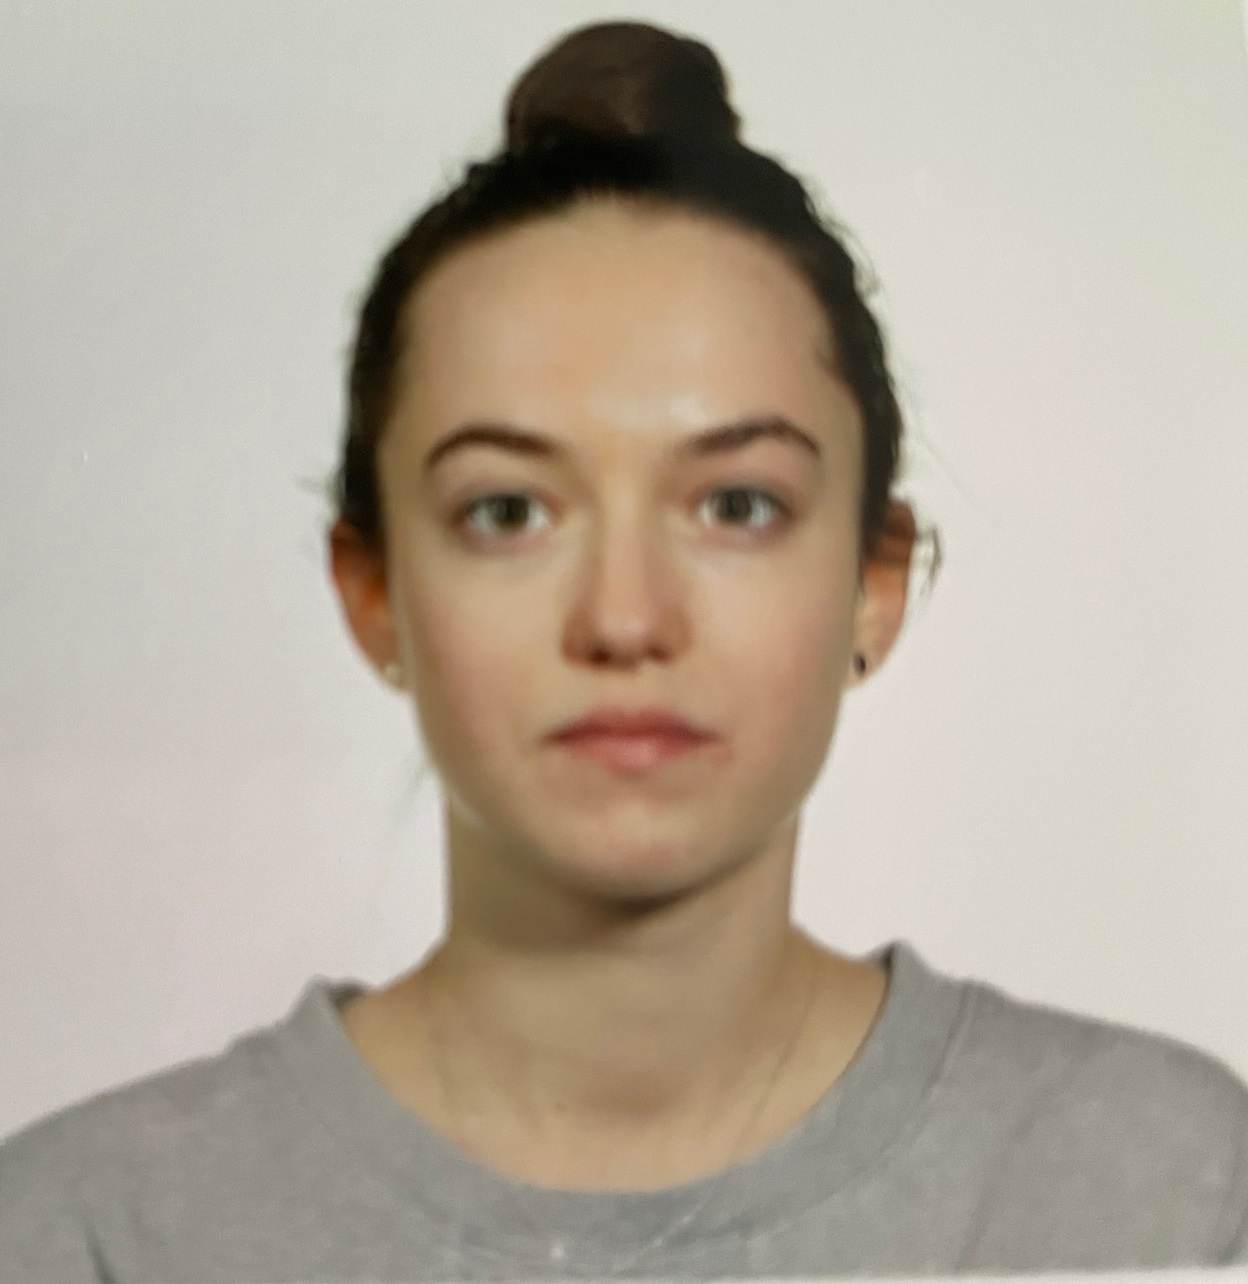
\includegraphics[width=0.6\columnwidth]{ma_photo.jpg}\\[\baselineskip] % Your photo
\small % Smaller font size
Charlotte Ayrault Christophe \\ % Your name
\url{charlotte.ayrault91@gmail.com} \\ % Your email address
07 85 66 18 32 \\ % Your phone number
\Sep % Some whitespace
\textbf{Address} \\
43 All\'ee du pont des beaunes \\ % Address 1
91120 Palaiseau  \\ % Address 2
\vfill % Whitespace under this block to push it up under the photo
\end{flushright}
}

%----------------------------------------------------------------------------------------

\begin{document}

\userinformation % Print your information in the left column

\framebreak % End of the first column

%----------------------------------------------------------------------------------------
%	HEADING
%----------------------------------------------------------------------------------------

\cvheading{Charlotte Ayrault Christophe} % Large heading - your name

\cvsubheading{\'Etudiante} % Subheading - your occupation/specialization

%----------------------------------------------------------------------------------------
%	ABOUT ME
%----------------------------------------------------------------------------------------

\aboutme{Profil}{A toi de remplir ici}

%----------------------------------------------------------------------------------------
%	EDUCATION
%----------------------------------------------------------------------------------------

\CVSection{Education}

%------------------------------------------------

\CVItem{2023 - 2019, Universit\'e Paris-Saclay} {Licence Math\'ematiques XX}

%------------------------------------------------

\CVItem{2019 - 2016, Lyc\'ee Fran\c{c}ais de New York (LFNY)}{Baccalaur\'eat XX}

%------------------------------------------------

\Sep % Extra whitespace after the end of a major section

%----------------------------------------------------------------------------------------
%	EXPERIENCE
%----------------------------------------------------------------------------------------

\CVSection{D\'etails \'education}

%------------------------------------------------

\CVItem{2019-2023, \textit{Licence Math\'ematiques}, Universit\'e Paris-Saclay}{
	\begin{itemize}
		\item Licence 1
		\begin{itemize}
			\item ALg\`ebre
			\item Physique
			\item G\'eom\'etrie des frises
		\end{itemize}
	\item Licence 2
		\begin{itemize}
			\item Alg\`ebre
			\item Analyse 
			\item Equations diff\'erentielles
			\item Probabilit\'e et statistique
			\item S\'ecurit\'e informatique
		\end{itemize}
	\item Licence 3
		\begin{itemize}
			\item Analyse Hilbertienne
			\item Analyse matricielle et optimisation
			\item Topologie et calcul diff\'erentiel
			\item Statistiques inf\'erentielles
		\end{itemize}
\end{itemize}

Langages informatiques
\begin{itemize}
	\item python
	\item R
\end{itemize}

Niveau anglais: B2 (IELTS)
}


\Sep % Extra whitespace after the end of a major section

%----------------------------------------------------------------------------------------
%	COMMUNICATION SKILLS
%----------------------------------------------------------------------------------------

\CVSection{Stages}

\CVItem{2016, \textit{Caisse des d\'epots}, Arcueil}{Pr\'esentation du service informatique et des activi\'es.}
\CVItem{2017, \textit{Systra}, New York}{Participation aux activit\'es du d\'epartement Marketing.}

\Sep % Extra whitespace after the end of a major section

%------------------------------------------------
\CVSection{Jobs d'\'et\'e}

\CVItem{2022, , Jardinerie Granville(50)}{Acceuil des clients, conseils et vente, soin des plantes.}
\CVItem{2021, , Super U Brehal (50)}{Information clients, r\'eapprovisionnements des rayons.}


\Sep % Extra whitespace after the end of a major section
%------------------------------------------------

\CVSection{Hobbies/Centres d'int\'er\^ets}

\CVItem{, \textit{Badmington}, LFNY et Universit\'e}{}
\CVItem{, \textit{Club cin\'ema, LFNY}}{}
\CVItem{, \textit{Cuisine}}{}

%------------------------------------------------


\end{document}
